% -*- tex-main-file: "contents.tex" compile-command: "pdflatex -halt-on-error p2p-private-cloud.tex > /dev/null" ispell-dictionary: "american" -*-

\NewScheme{\SPOR}{SPOR}

\subsection{\Acfp*{SPOR}}%
\label{sec:message_passing}

Say that Alice wants to send a message \(m\) to Bob.
Bob creates a reply header using \(\CreateReply\) and gives the output to Alice 
over an out-of-band channel.
We assume that \(m\) is either unavailable when the channel is used or too 
large to successfully send over the channel directly.
At a later point, Alice attaches a message \(m\) to the reply header using 
\(\UseReply\), creates a forward header using \(\CreateFwd\) with the prepared 
reply header as payload.
Then she sends this packet to the first node, which processes it using 
\(\ProcessHeader\).
The node will then process the header and in turn forward the packet to the 
next node.
At some point the message will reach Alice who identifies the message as the 
one expected to come from Bob.
(This process is illustrated in \cref{fig:file-exchange}.)
Now we will focus on how Alice and Bob choose the nodes that they provide to 
\(\CreateReply\) and \(\CreateFwd\).

\begin{figure}
  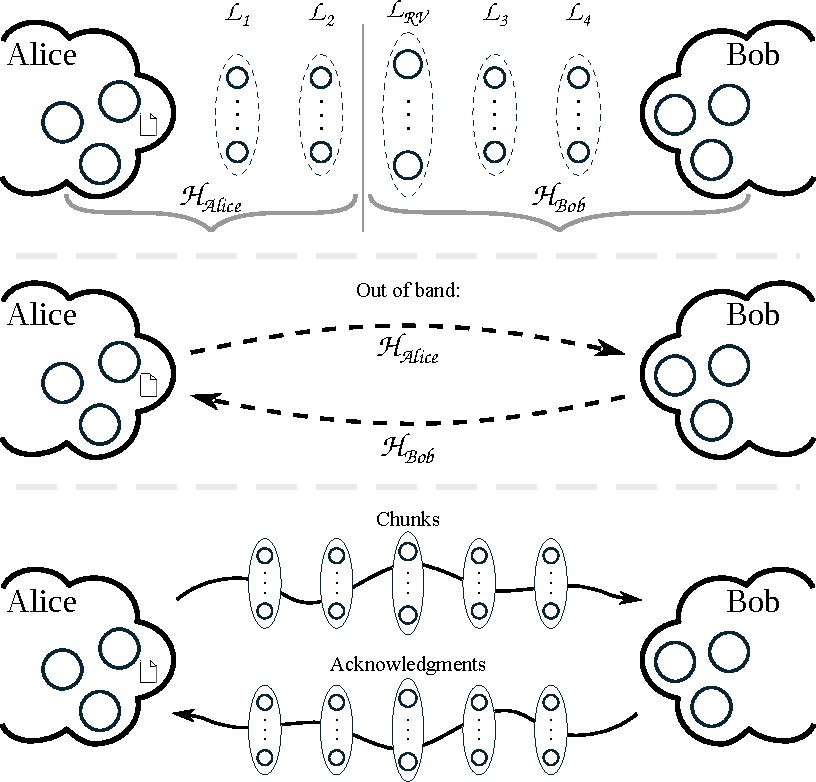
\includegraphics[width=\linewidth]{figures/file_exchange_v2.pdf}
  \caption{\label{fig:file-exchange}%
    A schematic of Alice and Bob sending a message using \name.
    \ding{1} illustrates the layer of the headers that Alice and Bob create.
    In \ding{2}, Alice and Bob exchange the headers out-of-band.
    In \ding{3}, Alice and Bob use two \ac{SPOR} routes, one for messages and 
    one for acknowledgements.
  }
\end{figure}

There are many uses of Sphinxes, many criteria that can be used to select the 
nodes in each layer.
We will focus on maximizing availability when routing in a network with high 
churn, but one could equally well select nodes to maximize, \eg, bandwidth.
We now describe a protocol, \ac{SPOR}, which uses Sphinxes to transfer messages 
from a source to a destination over a network of nodes with high churn.

\commentDaniel{We should describe how to do this selection using a prediction 
  oracle, then we provide a prediction oracle later.}

\subsection{\Acf*{SPORES}}

Above we made the usual assumption that Alice and Bob are represented by one 
device each.
Nowadays this is not the case: they both have multiple devices.
This means that Bob can receive Alice's message \(m\) on several alternative 
devices.
This might not be that problematic, so we will modify our scenario slightly:
The message \(m\) that Alice wants to send to Bob is too large to successfully 
pass every layer of the route.
\Eg each device goes offline and back online every \(t\) time units, the 
bandwidth is \(w\) size units per time unit and the message is \(l\) size 
units; if \(l\geq t w\), then the message \(m\) can never be delivered as any 
device will go offline before relaying it to the next node.
The natural solution is to split \(m\) into \(n\) parts, \(m_0, \dotsc, m_n\), 
where \(l/n\leq w t\).
The problem now is that \(m_i\) and \(m_j\) (\(i\neq j\)) might end up on 
different devices.

\commentDaniel{We should discuss this problem and outline our solution.}

